
\subsection{HDFS}
Hadoop use a distributed file system (HDFS) specialized for particular
types of applications. Files are stored as sets of blocks (64MB) which
are replicated for durability and availability.

\begin{center}
    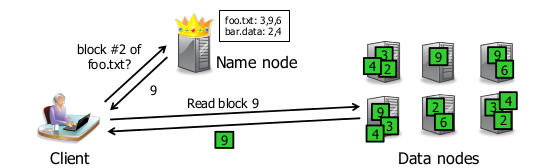
\includegraphics[width=11cm]{img/hdfs}
\end{center}

\begin{itemize}
    \item Namespace is managed by a single name node and transfert
        is done directly between client and data node
    \item State stored in two files:

        \begin{tabular}{m{7cm}m{9cm}}
            \begin{itemize}
                \item fsimages: snapshot of file system metadata
                \item edits: change since last snapshot
            \end{itemize} 
            &
            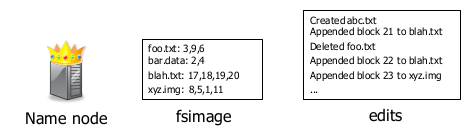
\includegraphics[width=9cm]{img/namenode}
        \end{tabular}
\end{itemize}
If the state of the namenode is lost, there are two possible solutions:
\begin{itemize}
	\item \textbf{Metadata backups} Namenode can write its metadata to a local disk
	and/or to a remote NFS
	\item \textbf{Secondary Namenode} (1) Periodically merge the edit log with fsimage 
	to prevent from growing to large, (2) Copy of the metadata
\end{itemize}
\paragraph{Note} Secondary namenode is more of a checkpoint
\footnote{http://blog.madhukaraphatak.com/secondary-namenode---what-it-really-do/} 
than a backup node, if it fails
$\to$ data loss.



\begin{table}[!h]
    \begin{tabular}{m{8cm}m{8cm}}
        \textbf{Does well} & \textbf{Does not well} \\
        \begin{itemize}
            \item very large read-only or append-only file (Terabytes EASY)
            \item Sequential access parten
            \item High throughput and high capacity
        \end{itemize} 
        &
        \begin{itemize}
            \item Low-latency access
            \item Multiple writers
            \item Not append-only file
            \item Storing small files
        \end{itemize} \\
        & $\rightarrow $ This is well done by Network File System (NFS)
    \end{tabular}
    \caption{HDFS advantage}
\end{table}


\subsection{Hive Query Language (HQL)}
A data warehouse infrastructure built on top 
of Hadoop for providing data summarization, 
query and analysis.

\subsubsection{SQL recap}
\begin{itemize}
    \item \texttt{SELECT}: Projection and remapping/renaming 
    \item \texttt{JOIN}: Cartesian product 
    \item \texttt{WHERE}: Filtering 
    \item \texttt{UNON, INTERSECT}: Set operations 
    \item \texttt{GROUP BY, MIN, MAX, AVG}: Aggregation 
    \item \texttt{ORDER BY}: Sorting 
    \item \texttt{SELECT .. FROM (SELECT .. FROM ..)}: Composition 
\end{itemize}

\subsubsection{HQL}

\begin{itemize}
    \item Suitable for processing structured data
    \item Create a table structure on top of HDFS
    \item Queries are compiled in to MapReduce jobs
\end{itemize}
\paragraph{Note} Hive is not designed fot OnLine Transaction Processing which 
consist mostly of updates. Indeed updating record or transaction are not 
supported

\subsection{Pig and Pig latin}
Relational data model does no allow nested table (attribute which is collection).
That's a part of what Pig Latin brings.

Somewhere between a programming language and a DBMSa which allows
distributed  programming with explicit parallel dataflow operators.

\begin{description}
    \item[Pig]: runtime system
    \item[Pig latin]:
        A dataflow language that compiles to MapReduce.
        Collection-­valued   expressions  whose  results  get  
        assigned  to  variables.
        \begin{itemize}
            \item A  program  does  a  series  of  assignments  in  a  dataflow
            \item It  gets  compiled  down  to  a  sequence  of  MapReduces. 

                Note that Pig Latin has its own query langage (not SQL)
        \end{itemize}

\end{description}

\subsubsection{Basic SQL-like operation}
Operations are \textbf{explicitly} specified.
\begin{itemize}
    \item \texttt{load\ldots as}: Projection and renaming 
    \item \texttt{foreach \ldots generate}: remapping 
    \item \texttt{filter by}: Filtering 
    \item \texttt{join}: intersection 
    \item \texttt{group by}: Aggregation 
    \item \texttt{order}: Sorting 
    \item \texttt{store}: save result
\end{itemize}

A Pig query can call functions that are written in Java

\subsubsection{Implementation}
\begin{center}
    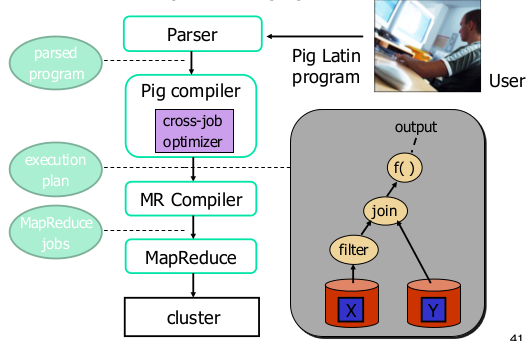
\includegraphics[width=10cm]{img/pig}
\end{center}

\subsubsection{Work-sharing techniques}
Use in order to reduce redundant work

\begin{center}
    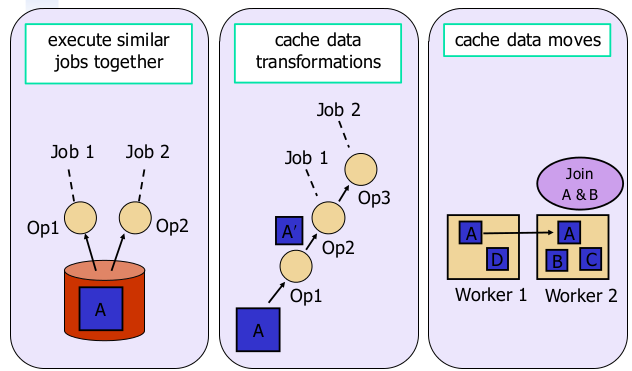
\includegraphics[width=10cm]{img/work}
\end{center}

\subsubsection{Example}
\begin{tabular}{m{9cm}m{6cm}}
    \begin{scriptsize}
    \begin{lstlisting}
Visits  =  load  '/data/visits'  as  (user,  url,  time);
Visits  =  foreach Visits  generate  user,  Canonicalize(url),  time;

Pages  =  load  '/data/pages'  as  (url,  pagerank);
VP  =  join  Visits  by  url,  Pages  by  url;
UserVisits =  group  VP  by  user;
Sessions  =  foreach UserVisits generate
flatten(FindSessions(*));
HappyEndings =  filter  Sessions  by  BestIsLast(*);

store  HappyEndings into  '/data/happy_endings';
\end{lstlisting}
    \end{scriptsize}
&
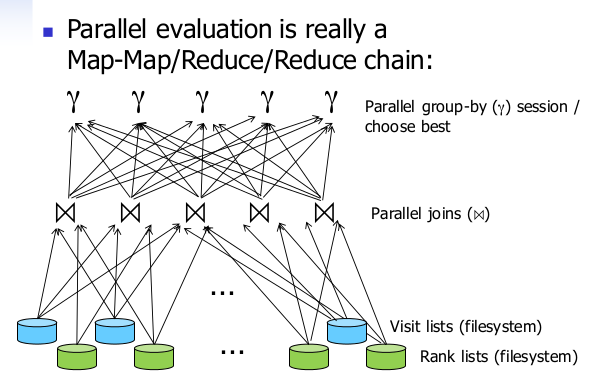
\includegraphics[width=7cm]{img/pigg}
\end{tabular}


